\section{提案手法} \label{sec3}
\begin{figure}[tb]
\centerline{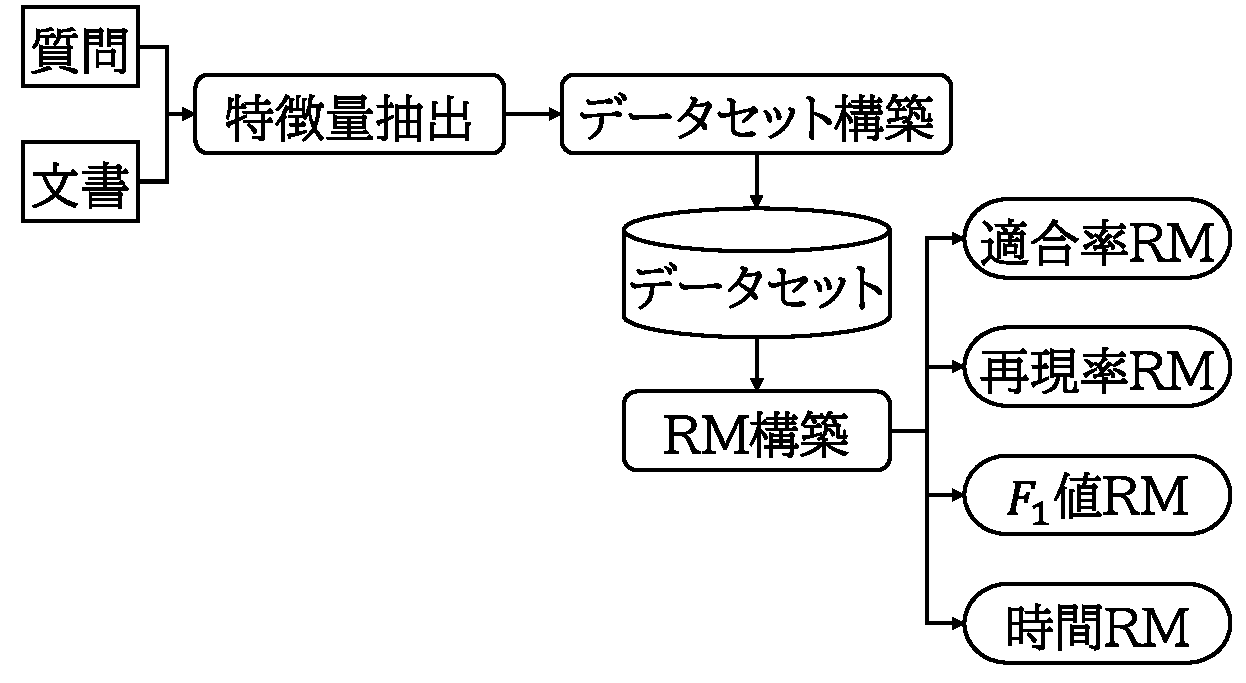
\includegraphics[width=\linewidth]{figures/method_construction_diagram.pdf}}
\caption{提案手法におけるランキングモデルの学習手順}
\label{construction}
\end{figure}

\begin{figure}[tb]
\centerline{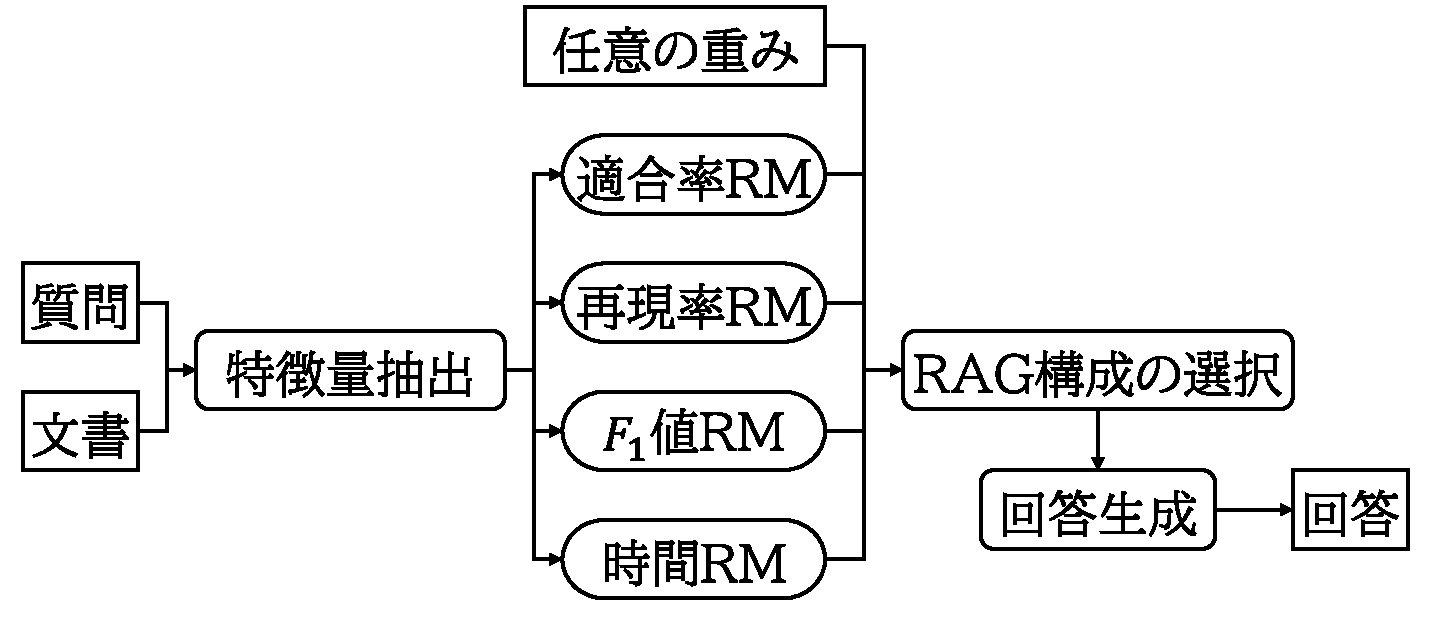
\includegraphics[width=\linewidth]{figures/method_reasoning_diagram.pdf}}
\caption{提案手法におけるランキングモデルの推論手順}
\label{reasoning}
\end{figure}

本研究では，質問と文書の特徴に応じてRAG構成を適応的に選択し，精度（適合率・再現率・$F_1$値）とコスト（実行時間）のトレードオフを調整する手法を提案する．
\ref{construction}および~\ref{reasoning}に，提案手法におけるRMの学習と推論の手順を示す．
%提案手法は，ランキングモデルの学習とランキングモデルによる推論により構成される．
% \ref{construction}および~\ref{reasoning}における適合率RM，再現率RM，$F_1$値RM，時間RMは，それぞれ適合率，再現率，$F_1$値，時間のRMを表す．
適合率RM，再現率RM，$F_1$値RM，時間RMは，質問と文書の特徴量とRAG構成を説明変数として用いる．
これらは，各RAG構成における適合率，再現率，$F_1$値，および実行時間の順位をそれぞれ予測するモデルである．
本章では，提案手法におけるRMの学習および推論の構成要素について述べる．

\subsection{特徴量抽出} \label{sec3.1}
本節では，質問および文書から表層的特徴量と意味的特徴量を抽出する方法を説明する． 
あらかじめ質問に関連する文書を一つ以上用意した上で，本処理はRMの学習と推論の双方で実行する． 
これらの特徴量は，質問の複雑さと意図，および質問と文書の関連性を捉えるために用いる． 
特徴量は，表層的特徴量4種類と意味的特徴量3種類の計7種類を選定した．
この選定は，事前に様々な特徴量の組み合わせを試し，RMの性能が最も向上する組を特定するというヒューリスティックな手法に基づいている．
なお，性能評価の詳細については，第~\ref{sec5.5}のアブレーション分析にて述べる．
% 特徴量は，ヒューリスティックな手法により，表層的特徴量4種類と意味的特徴量3種類の計7種類を選定した． 

\subsubsection{表層的特徴量の抽出}
表層的特徴量は，質問に関するトークン数，依存構造木の深さ，質問タイプ，および文書に関するトークン数の4種類である． 
質問のトークン数は，質問の表層的な長さを表すだけでなく，複数の条件，制約，あるいは修飾句を含む可能性を反映する指標である．
一般に，質問が長いほど，回答に必要な根拠が単一文書に収まらず，複数文書の統合を要する場合が増加する．

質問の依存構造木の深さは，トークン同士の係り受け関係を有向木として表現し，ルートトークンから深さ優先探索をした際の到達可能なパス長である．
木構造が深いほど修飾の入れ子や長距離依存が多く，文の解釈に必要な統合を要する場合が増加する．
RAG の構成選択の観点では，構文が複雑な質問ほど複数文書に跨る情報の統合を必要とする．

質問タイプは，期待される出力に基づき，真偽判定（Yes/No），本文抽出（事実情報の特定），選択（提示候補からの選定），文章生成（自由記述による説明）の4種類に分類する．
判定には，質問文の小文字化により得られた先頭語および特定語に基づくルールベースを採用する．
先頭語がis，can，mustといった助動詞やbe動詞である場合は，事象の成立可否を問う性質を持つため「真偽判定」に分類する．
一方，先頭語がwhat，who，whereといった疑問詞は，具体的な情報の特定を促すため「本文抽出」に分類する．
質問文に特定語（or）を含む場合は，選択を促す「選択」に分類する．
これら全条件に該当しない質問は，要約や理由説明の記述が求められるとみなし，「文章生成」に分類する．
% まず，真偽判定を促す語群（is, are, can, could, will, would, has, have, had, shall, should, may, might, must），選択を促す語（or），本文抽出を促す語群（what, who, when, where, which）のいずれに該当するかに基づいて，真偽判定，選択，本文抽出のいずれかに分類する．
% その他を説明生成や要約といった自由度の高い出力が求められるとみなし，文章生成に分類する．

文書に関するトークン数は，含まれる情報量の多さを示すと同時に，冗長性やノイズ量の増加を示唆する．
特に文書が長い場合，適切なチャンク分割の調整や検索後の統合手法の選択が性能およびコストに影響するため，本特徴量は構成選択に有用である．

\subsubsection{意味的特徴量の抽出}
意味的特徴量は，質問と文書の各埋め込み間のコサイン類似度，質問と文書から抽出したキーワードとの類似度，および質問と文書の双方から抽出した固有表現のコサイン類似度の3種類である．
質問と文書の各埋め込み間のコサイン類似度は，大域的な意味の一致度を測る指標であり，類似度が高い場合単一文書が回答根拠になり得る可能性が高く，比較的単純なRAG構成でも回答可能であると判断できる．

質問と文書から抽出したキーワードとの類似度は，質問と文書から抽出した語句を連結した文字列との類似度である．
文書は冗長な周辺情報を含みやすく，長文では質問に関連する箇所が埋もれる場合がある．
キーワードを用いることで要点レベルの整合性を判断する．
% そこで，文書からキーワードを抽出し，質問文との意味的近接性を測ることで要点レベルの整合性を評価する．

質問と文書の双方から抽出した固有表現のコサイン類似度は，質問および文書から抽出された固有表現の文字列を比較するものである．
固有表現は人物，組織，地名，作品名などの参照対象を表し，質問応答の品質を左右する要因となる．

以上の三つのコサイン類似度は，全文レベル，要点レベル，エンティティレベルという異なる観点から，質問と文書の関連性を補完的に捉えるものである．

\subsection{データセット構築} \label{sec3.2}
本節ではRMの学習，検証および評価に用いるデータセットの構築について述べる．
広範な構成空間から精度とコストの分布を系統的に取得し，RMが構成選択の規則性を学習する．
各質問に対して想定される全てのRAG構成を適用し，高精度な構成や低コストな構成を相対比較可能な順位ラベルを付与する．

RAG構成は，\ref{hyperparameters_in_RAG} に示す6項目の組み合わせからなる96通りに設定する．
RAGはNaiveRAG~\cite{Lewis20}，LightRAG~\cite{Guo25}，およびGraphRAG~\cite{edge25}を用いる． 
検索設定（Retrieval Setting, RS）は，NaiveRAGではStuffまたはMap Reduceとし，LightRAGおよびGraphRAGではローカル検索（Local）またはグローバル検索（Global）とする． 
チャンク設定は，NaiveRAGではチャンクサイズ（Chunk Size, CS）を250または500，チャンクオーバーラップ（Chunk Overlap, CO）を50または100とする． 
LightRAGおよびGraphRAGでは，CSを500または1000，COを100または250とする．
生成モデル（Generative Model, GM）には，Llama3.1:8b~\cite{Meta24}とQwen3:14b~\cite{qwen25} を用い，埋め込みモデル（Embedding Model, EM）にはnomic-embed-text~\cite{nussbaum25}とmxbai-embed-large~\footnote{\url{https://www.mixedbread.com/blog/} \url{mxbai-embed-large-v1/}}を用いる．
これにより多様な構成を網羅し，RM学習に必要な性能差を確保する．

なお，本研究では3種類のRAGを横断して比較可能な学習データを構築するため，構成の種類を可能な限り統一した．
% ただし，各RAGの構成は必ずしも同一ではない．
そのため，検索設定だけでなく，検索情報の統合方針（Chain Type）も広義の「検索設定」として扱う．
NaiveRAGにおけるChain Typeを，LightRAGおよびGraphRAGにおける検索設定と見なす．
本論文では，これらを統一して「検索設定」と記述する．

次に，各試行の結果として，質問 ID，RAG 構成，適合率，再現率，$F_1$値，実行時間を記録し，RMの特徴量と結合してデータセットを作成する．
具体的には，質問と文書を各 RAG 構成に入力し，得られた生成回答と正解を比較して BERTScore~\cite{zhang20}に基づく適合率・再現率・$F_1$ 値を算出する．
同時に，コストの指標として各試行の実行時間を計測する．
BERTScore は語彙の完全一致に依存せず，文脈埋め込みに基づいてトークン間の意味的対応を定量化できる．
そのため，表現の揺れを含む生成回答の評価に適している．
適合率，再現率，$F_1$値，実行時間には，相対的な順位を付与する．

% \begin{table*}[tb]
%     \centering
%     \small
%     % \footnotesize
%     \caption{RAG構成}
%     \label{hyperparameters_in_RAG}
% %    \resizebox{\columnwidth}{!}{
%     \begin{tabular}{cccccc}
%         \hline
%         \multirow{2}{*}{RAG} & \multirow{2}{*}{検索設定}
%         & \multicolumn{2}{c}{チャンク} & \multicolumn{2}{c}{モデル} \\
%         && サイズ & OL & 生成 & 埋め込み \\
%         \hline
%         \multirow{2}{*}{NaiveRAG} 
%         & Stuff & 250 & 50 & llama3.1:8b & nomic-embed-text \\
%         & MR & 500 & 100 & qwen3:14b & mxbai-embed-large \\
%         \hline
%         \multirow{2}{*}{LightRAG} 
%         & Local & 500 & 100 & llama3.1:8b & nomic-embed-text \\
%         & Global & 1000 & 250 & qwen3:14b & mxbai-embed-large \\
%         \hline
%         \multirow{2}{*}{GraphRAG} 
%         & Local & 500 & 100 & llama3.1:8b & nomic-embed-text \\
%         & Global & 1000 & 250 & qwen3:14b & mxbai-embed-large \\
%         \hline
%     \end{tabular}
% %    }
% \end{table*}

\begin{table}[tb]
    \centering
    \small
    % \footnotesize
    \caption{RAG構成（全96通りの組み合わせ）}
    \label{hyperparameters_in_RAG}
    \begin{tabular}{lll}
        \hline
        構成 & 対象RAG & 設定値 \\
        \hline
        \multirow{2}{*}{RAG} & - & \{NaiveRAG, LightRAG, \\ &&GraphRAG\} \\
        \hline
        \multirow{2}{*}{RS} & NaiveRAG & \{Stuff, Map Reduce\} \\ 
        & LightRAG / GraphRAG & \{Local, Global\} \\
        \hline
        \multirow{2}{*}{CS} & NaiveRAG & \{250, 500\} \\ 
        & LightRAG / GraphRAG & \{500, 1000\} \\
        \hline
        \multirow{2}{*}{CO} & NaiveRAG & \{50, 100\} \\ 
        & LightRAG / GraphRAG & \{100 , 250\} \\
        \hline
        \multirow{2}{*}{GM} & \multirow{2}{*}{全RAG共通} 
        & \{llama3.1:8b, \\ && qwen3:14b\} \\
        \hline
        \multirow{2}{*}{EM} & \multirow{2}{*}{全RAG共通} 
        & \{nomic-embed-text, \\ && mxbai-embed-large\} \\
        \hline
    \end{tabular}
\end{table}

\subsection{ランキングモデル学習} \label{sec3.3}
本節では，\ref{sec3.2}で構築したデータセットを用いて，RAG構成の順位を予測するRMを学習する手順を述べる．
本手法は，新規質問に対して直接RAG構成や評価指標の値を当てるのではなく，同一質問に対する複数候補間の相対的な優劣を予測する点が特徴である．
これにより，回帰手法で懸念される質問の難易度によるスコアの絶対値変動や計測ノイズの影響を抑制し，頑健な学習が可能となる．
さらに，分類手法で懸念されるラベル不均衡や順位情報の欠落を回避し，上位候補を精度よく識別するという本研究の目的に直結したRM学習が実現できる．
RMの説明変数には6種類のRAG構成も使用するため，7個の特徴量と6個のRAG構成の合計13個が説明変数となる．
RMの目的変数は，適合率，再現率，$F_1$値，実行時間といった評価観点ごとに学習する．
これは，精度とコストの重要度が利用目的により変化し得るためである．
推論時には，それぞれの観点に対して予測順位を得たうえで，\ref{sec3.4}で述べる総合評価値により最終構成を選択する．
この分離設計により，特定の観点用の単一モデルに依存せず，ユーザが指定する重みに応じて意思決定を柔軟に切り替えられる．

\subsection{RAG構成の選択} \label{sec3.4}
本節ではRAG構成の選択について述べる． 
% \newpage %行間調整用
\ref{reasoning}に示す通り，新規の質問と文書が入力されると特徴量を抽出し，RMによって各評価指標における各RAG構成の順位を予測する．
式~\eqref{eq1}により総合評価値を算出し，最も高いスコアを与える構成を採用する．
\begin{equation}\begin{aligned}
総合評価値
=  \frac{W_{\mathrm{pre}}}{P_{\mathrm{rank}}}
+ \frac{W_{\mathrm{rec}}}{R_{\mathrm{rank}}}
+ \frac{W_{\mathrm{f_1}}}{{F_1}_{\mathrm{rank}}}
+ \frac{W_{\mathrm{time}}}{T_{\mathrm{rank}}}
\label{eq1}
\end{aligned}\end{equation}
ただし，重みは式~\eqref{eq2}の制約を設ける．
\begin{equation}\begin{aligned}
W_{\mathrm{pre}} + W_{\mathrm{rec}} + W_{\mathrm{f_1}} + W_{\mathrm{time}} = 1
\label{eq2}
\end{aligned}\end{equation}

ここで，$P_{\mathrm{rank}}$，$R_{\mathrm{rank}}$，${F_1}_{\mathrm{rank}}$および$T_{\mathrm{rank}}$はそれぞれ適合率，再現率，$F_1$値，実行時間の予測値に基づく順位を表す．
各項において順位の逆数を用いることで，より上位の性能を持つ手法に対し，高いスコアを与える設計とする．
最終的に，最大の総合評価値を得た RAG 構成を回答生成に用いる．
